\Subhead{6.3.3}{Выделение сигнала из шума. Согласованный фильтр}

Пусть известный детерминированный импульс $s(t)$ действует на фоне стационарного шума со спектром $S_n(\omega)>0$. На выходе линейного фильтра в выбранный момент $t_0$
\begin{equation}
 s_o(t_0)=\frac1{2\pi}\int H(\omega)S(\omega)\e^{-\ii\omega t_0}\dd\omega,\quad
 \sigma_o^2=\frac1{2\pi}\int|H|^2S_n\dd\omega.
\end{equation}
Применение Коши–Буняковского к $H\sqrt{S_n}$ и $S^*\e^{\ii\omega t_0}/\sqrt{S_n}$ показывает, что максимум $|s_o|^2/\sigma_o^2$ достигается при
\begin{equation}\label{eq:matched}
 H(\omega)=C\frac{S^*(\omega)\e^{\ii\omega t_0}}{S_n(\omega)},
 \qquad \mathrm{SNR}_{\max}=\frac1{2\pi}\int\frac{|S(\omega)|^2}{S_n(\omega)}\dd\omega.
\end{equation}
При белом шуме $S_n=N_0/2$ импульсная характеристика $h(t)\propto s(t_0-t)$ для вещественного сигнала, а максимум SNR равен $2E_s/N_0$, $E_s=\int s^2\dd t$. Это коррелятор со сдвинутым обращённым шаблоном. Задержка $t_0$ должна позволять причинную реализацию конечного импульса; бесконечный шаблон не становится строго причинным одним названием.

В окрашенном шуме формула~\eqref{eq:matched} задаёт оптимум \emph{без ограничения причинности}. Обратное преобразование $1/S_n$ может иметь бесконечный хвост при отрицательных временах, который не устраняется конечной задержкой. Например, при $S_n=N[1+\eta/(1+\omega^2\tau_c^2)]$, $N,\eta>0$, оно содержит член $\propto-\exp[-\sqrt{1+\eta}|t|/\tau_c]$. Для приёма к заданному сроку надо учитывать доступный интервал наблюдений и причинную факторизацию/отбеливание, как в~\Qref{6.3.2}. Спектрально шумные компоненты подавляются, затем выполняется согласование.
% Контрпример: 1/S_n=N^{-1}[1-eta/(1+eta+omega^2 tau_c^2)],
% обратное преобразование второго члена двусторонне; конечный сдвиг хвост не убирает.

Для гауссовского шума та же статистика возникает в отношении правдоподобий, поэтому пороговый согласованный приём оптимален для известного сигнала при заданном критерии обнаружения. При неизвестной фазе нужны квадратурный/энергетический вариант и соответствующее распределение статистики. Нормировка фильтра не меняет SNR, но меняет численный порог.
\begin{center}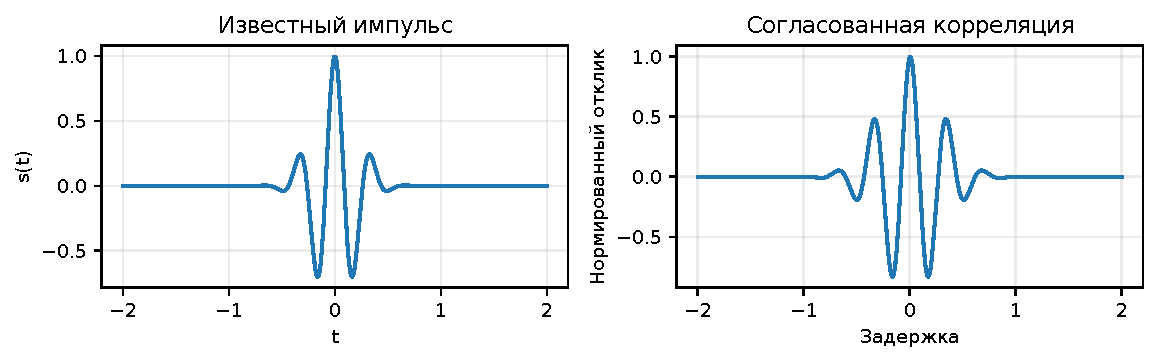
\includegraphics[width=0.8\linewidth]{figures/matched.pdf}\end{center}

